% !TEX root = ../vr_st.tex

%Let $X$ be an $\R$-space where $X_r$ is empty for $r<0$ and contractible for $r\geq R$ for some real number $R$.
%The Vietoris--Rips complex of a metric space is our primary example.
%In this subsection, we will consider this $\R$-space and omit it from the notation when convenient.

\subsection{Kuratowski embedding and critical radii}\label{sub:filling radii}

\subsubsection{}

Any compact metric space $\cX$ can be isometrically embedded into the space $\rL^\infty(\cX)$ of all bounded real-valued functions on $\cX$ via the map $x \in \cX \mapsto d_\cX(x,\cdot)$, the so-called \defn{Kuratowski embedding}.
We are interested in the \(\R\)-space obtained by considering radius \(r\) neighborhoods of the image of \(\cX\), which we denote \(\rU_r(\cX)\).

Throughout the text, Riemannian manifolds are thought of as metric spaces with the geodesic distance.

\subsubsection{}\label{ss:kuratowski_vr}

As proven in \cite[Thm.~4.1]{lim2024vietoris}, there is deep relationship between the \(r\)-neighborhood filtration of $\cX$ in $\rL^\infty(\cX)$ and the Vietoris--Rips complex of \(\cX\) at scale \(2r\), stated in the following.

\medskip\proposition The spaces $\VR_{2r}(\cX)$ and $\rU_r(\cX)$ are naturally homotopy equivalent for every \(r > 0\).

\subsubsection{}

Following \cite{gromov1983filling}, the \defn{filling radius} of an \(n\)-dimensional closed orientable Riemannian manifold $\cM$, denoted \(\fillrad(\cM)\), is defined as the infimal $\epsilon > 0$ such that the fundamental class in $\rH_n(M; \Z)$ is mapped to zero by the inclusion $\cM \hookrightarrow \rU_\epsilon(\cM)$, where \(\rU_\epsilon(\cM)\) is the \(\epsilon\)-neighborhood of \(\cM\) in \(\rL^\infty(\cX)\).
This definition can be generalized by considering different homology coefficients.
That is,
\[
\fillrad(\cM; \field) = \min\set[\big]{r \mid (0, r) \in \barc \rH_n(\rU(\cM); \field)}.
\]

For non-orientable manifolds, the filling radius is defined similarly using \(\Ftwo\) coefficients.

\subsubsection{}

The natural homotopy equivalence described in \cref{ss:kuratowski_vr} implies
\[
\fillrad(\cM; \field) = \min\set[\big]{r \mid (0, 2r) \in \barc \rH_n(\VR(\cM); \field)}.
\]
Moreover, it gives rise to the following result proven in \cite[Prop.~9.28]{lim2024vietoris}.

\medskip\lemma
If $\cM$ is a closed connected $n$-dimensional Riemannian manifold, then \(\Hbarc{n}{\cM}\) contains the bar \((0,2\fillrad(\cM))\) for arbitrary field coefficients if $M$ is orientable, and for mod $2$ coefficients $M$ if not.
Moreover, this is the unique bar in \(\Hbarc{n}{\cM}\) starting at $0$.

\subsubsection{}\label{ss:first_critical_value}

Let \(\cM\) be a closed Riemannian manifold.
By \cite[Thm.~3.5]{hausmann1995vietoris} and \cite[Thm.~4.1]{lim2024vietoris}, we know that there exists \(r_\cM > 0\) such that for all \(r \in (0, r_\cM)\) the inclusion \(\cM \to \VR_{2r}(\cM)\) is a homotopy equivalence.
We define the \defn{homotopical radius} of \(\cM\), denoted by \(\crit(\cM)\), as the supremum among all such real numbers.

\subsubsection{}

Let us fix a field \(\field\) and an integer \(m \in \N\), the \defn{\(m\)-homological radius} of a totally bounded metric space \(\cX\) is defined by
\[
\firstdeath{m}{\cX; \field} = \min\set[\big]{r \mid (0, 2r) \in \barc \rH_m(\VR(\cX); \field)},
\]
if \(\rH_\degp(\cX) \neq 0\).
If \(\rH_\degp(\cX) = 0\), set \(\firstdeath{m}{\cX} = 0\).
We will omit \(\field\) from the notation when clear from the context.

Similarly, for a linear cohomology operation \(\theta\), we define the \defn{\(\img_\theta\)-radius} of \(\cX\) by
\[
\firstdeath{\theta}{\cX} = \min\set[\big]{r \mid (0, 2r) \in \barc \img_\theta(\VR(\cX))},
\]
if \(\img_\theta(\cX) \neq 0\).
If \(\img_\theta(\cX) = 0\), set $\firstdeath{\theta}{\cX} = 0$.

The \(\ker_\theta\)-radius could be defined similarly, but we do not use it in this work.

\anibal{Please study this label: \{subsub:beta v.s. fillrad\}. I.e., where is it used and what to cite instead.
\ling{The label is needed to refer to what is commented out below. I brought them back and added the label back too.
}}

\subsubsection{}
\label{ss:beta v.s. fillrad}

Clearly, if \(\rH_m(\cX) \neq 0\) (resp. \(\img_\theta(\cX) \neq 0\)), then
\[
    \crit(\cX) \leq \firstdeath{m}{\cX} \qquad (\text{resp. }\crit(\cX) \leq  \firstdeath{\theta}{\cX}),
\]
and if $\cM$ is connected and $n$-dimensional, then
\[\firstdeath{n}{\cM} = \fillrad(\cM).\]

%\subsubsection{}

%Let us assume \(\cM\) connected.
%Since, as stated in \cref{ss:kuratowski_vr}, \(\VR_{2r}(\cM)\) is homotopy equivalent to \(U_r(\cM) \subset \rL^\infty(\cM)\), an upper bound for \(\crit(\cM)\) is \(2\cdot\Rad(\cM)\).
%
%We generalize this from the top homology to every other degree \(\degp\) and to non-connected manifolds so that
%\[
%\Rad_\degp(\cM) = \Rad(\cM)
%\]
%if \(\cM\) is connected and \(\degp\)-dimensional.


\subsection{General estimates}\label{ss:barcode_general}

Let \(\cM\) be a closed Riemannian manifold. 
Consider \(\ell, \degp \in \N\) and \(\theta \in \cO(\ell,\degp)\).
We will simplify notation writing \(R = \diam(\cM),\, \alpha = 2\crit(\cM)\), \(\beta_m = 2\firstdeath{\degp}{\cM}\), and \(\gamma_\theta = 2\firstdeath{\theta}{\cM}\). 
We say a bar $(a, b)$ is \defn{dominated} by another $(c,d)$ if $c \leq a < b \leq d$.

Because $\VR_r(\cM)$ is empty for \(r \leq 0\) and the homotopy type of $\VR_r(\cM)$ remains the homotopy type of $\cM$ for $r \in (0, \alpha)$, bars in \(\barc \rH_\degp^{\VR}(\cM)\) and $\barc\img_\theta^{\VR}(\cM)$ either start at $0$ or start after $\alpha$.

More precisely,
%we estimate the reduced homology barcode of $\cM$ by considering two cases.
if \(k = \dim \opH_\degp(\cM) > 0\) then $\barc\rH_\degp^{\VR}(\cM)$ contains $(0, \beta_m)$ and \((k - 1)\) additional bars of the form \((0, b)\) with \(\beta_m \leq b \leq R\).
Additionally, all other bars are dominated by \((\alpha, R)\).
If \(\dim \opH_\degp(\cM) = 0\) then all bars in \(\barc\rH_\degp^{\VR}(\cM)\) are dominated by \((\alpha, R)\).
See the first row of \cref{fig:barcodes_general} for a pictorial representation of these estimates.

A similar analysis applies to $\barc\img_\theta^{\VR}(\cM)$.
See the second row of \cref{fig:barcodes_general} for these estimates.

\begin{figure}
	\centering
	\begin{tikzpicture}[scale=0.52]
	\begin{axis} [
		title = {\LARGE $\barc\opH_m^{\VR}(\cM)$, if $\opH_m(\cM) \neq 0$},
		ticklabel style = {font=\Large},
		axis y line=middle,
		axis x line=middle,
		ytick={0.7,0.95},
		yticklabels={$2\firstdeath{m}{\cM}$,$\diam(\cM)$},
		xtick={0.55,0.95},
		xticklabels={$2\crit(\cM)$, $\diam(\cM)$},
		xmin=-0.015, xmax=1.1,
		ymin=0, ymax=1.1,]
		\addplot [mark=none] coordinates {(0,0) (1,1)};
		\addplot [thick,color=black!20!white,fill=black!30!white,
		fill opacity=0.4]coordinates {
			(0.55,0.95)
			(0.55,0.55)
			(0.95,0.95)
			(0.55,0.95)};
		\addplot [black!40!white,mark=none,dashed, thin] coordinates {(0,0.7) (0.7,0.7)};
		\addplot [black!40!white,mark=none,dashed, thin] coordinates {(0,0.55) (0.55,0.55)};
		\addplot [black!40!white,mark=none,dashed, thin] coordinates {(0.55,0) (0.55,0.55)};
		\addplot[line width=1.5mm, color=black!30!white] coordinates{(0, 0.7) (0, 0.95)};
		\addplot[barccolor,mark=*] (0, 0.7) circle (2pt) node[above right,barccolor]{};
	\end{axis}
\end{tikzpicture}
\begin{tikzpicture}[scale=0.52]
	\begin{axis} [
		title = {\LARGE $\barc\opH_m^{\VR}(\cM)$, if $\opH_m(\cM) = 0$},
		ticklabel style = {font=\Large},
		axis y line=middle,
		axis x line=middle,
		ytick={0.95},
		yticklabels={$\diam(\cM)$},
		xtick={0.55,0.95},
		xticklabels={$2\crit(\cM)$, $\diam(\cM)$},
		xmin=-0.015, xmax=1.1,
		ymin=0, ymax=1.1,]
		\addplot [mark=none] coordinates {(0,0) (1,1)};
		\addplot [thick,color=black!20!white,fill=black!30!white,
		fill opacity=0.4]coordinates {
			(0.55,0.95)
			(0.55,0.55)
			(0.95,0.95)
			(0.55,0.95)};
		\addplot [black!40!white,mark=none,dashed, thin] coordinates {(0,0.55) (0.55,0.55)};
		\addplot [black!40!white,mark=none,dashed, thin] coordinates {(0.55,0) (0.55,0.55)};
	\end{axis}
\end{tikzpicture}

\begin{tikzpicture}[scale=0.52]
	\begin{axis} [
		title={\LARGE $\thetabarc{\cM}$, if $\img\theta_{\cM}\neq 0$},
		ticklabel style = {font=\Large},
		axis y line=middle,
		axis x line=middle,
		ytick={0.7,0.95},
		yticklabels={$2\firstdeath{\theta}{\cM}$,$\diam(\cM)$},
		xtick={0.55,0.95},
		xticklabels={$2\crit(\cM)$, $\diam(\cM)$},
		xmin=-0.015, xmax=1.1,
		ymin=0, ymax=1.1,]
		\addplot [mark=none] coordinates {(0,0) (1,1)};
		\addplot [thick,color=black!20!white,fill=black!30!white,
		fill opacity=0.4]coordinates {
			(0.55,0.95)
			(0.55,0.55)
			(0.95,0.95)
			(0.55,0.95)};
		\addplot [black!40!white,mark=none,dashed, thin] coordinates {(0,0.7) (0.7,0.7)};
		\addplot [black!40!white,mark=none,dashed, thin] coordinates {(0,0.55) (0.55,0.55)};
		\addplot [black!40!white,mark=none,dashed, thin] coordinates {(0.55,0) (0.55,0.55)};
		\addplot[line width=1.5mm, color=black!30!white] coordinates{(0, 0.7) (0, 0.95)};
		\addplot[barccolor,mark=*] (0, 0.7) circle (2pt) node[above right,barccolor]{};
	\end{axis}
\end{tikzpicture}
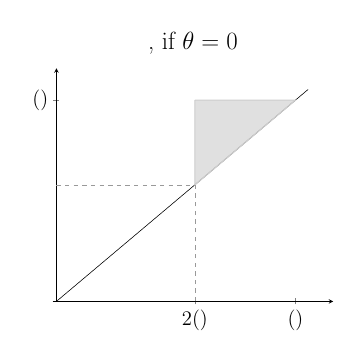
\begin{tikzpicture}[scale=0.52]
	\begin{axis} [
		title={\LARGE $\thetabarc{\cM}$, if $\img\theta_{\cM}= 0$},
		ticklabel style = {font=\Large},
		axis y line=middle,
		axis x line=middle,
		ytick={0.95},
		yticklabels={$\diam(\cM)$},
		xtick={0.55,0.95},
		xticklabels={$2\crit(\cM)$, $\diam(\cM)$},
		xmin=-0.015, xmax=1.1,
		ymin=0, ymax=1.1,]
		\addplot [mark=none] coordinates {(0,0) (1,1)};
		\addplot [thick,color=black!20!white,fill=black!30!white,
		fill opacity=0.4]coordinates {
			(0.55,0.95)
			(0.55,0.55)
			(0.95,0.95)
			(0.55,0.95)};
		\addplot [black!40!white,mark=none,dashed, thin] coordinates {(0,0.55) (0.55,0.55)};
		\addplot [black!40!white,mark=none,dashed, thin] coordinates {(0.55,0) (0.55,0.55)};
	\end{axis}
\end{tikzpicture}
	\caption{Let $\cM$ be a closed Riemannian manifold.
    \emph{Top row:} persistent reduced homology barcodes of $\cM$.
	\emph{Bottom row:} $\img_\theta$-barcodes of $\cM$.
    In each figure, the gray region represents where additional bars could potentially exist within the corresponding barcode.
    See \cref{ss:barcode_general} for details.}
	\label{fig:barcodes_general}
\end{figure}